\documentclass[11pt,a4paper]{article}

\usepackage[utf8]{inputenc}
\usepackage[T1]{fontenc}
\usepackage{lmodern}
\usepackage{amsmath,amssymb,amsfonts}
\usepackage{graphicx}
\usepackage{hyperref}
\usepackage{xcolor}
\usepackage{booktabs}
\usepackage{listings}
\usepackage{float}
\usepackage{algpseudocode}
\usepackage{tikz}
\usepackage[ruled,vlined]{algorithm2e}

\hypersetup{
    colorlinks=true,
    linkcolor=blue,
    filecolor=magenta,
    urlcolor=cyan,
}

\title{Paper Bridge Finder: Discovering Connections Between Research Areas}
\author{Your Name}
\date{\today}

\begin{document}

\maketitle

\begin{abstract}
This report presents the Paper Bridge Finder, a system designed to identify academic papers that connect different research domains. By leveraging natural language processing, graph theory, and machine learning techniques, the system builds a knowledge graph of papers and topics, then identifies papers that serve as bridges between distinct research areas. The system includes components for data ingestion, embedding generation, topic modeling, knowledge graph construction, and bridge paper ranking. Experimental results demonstrate the system's ability to discover meaningful connections between research fields, potentially accelerating interdisciplinary research and collaboration.
\end{abstract}

\tableofcontents
\newpage

\section{Executive Summary}

The Paper Bridge Finder is a novel system that addresses the challenge of discovering connections between seemingly disparate research areas. In the increasingly specialized academic landscape, finding papers that effectively bridge different domains is crucial for interdisciplinary research but often difficult and time-consuming.

Our system automates this discovery process by:
\begin{itemize}
    \item Ingesting paper metadata from academic repositories (arXiv, Semantic Scholar)
    \item Generating semantic embeddings of paper abstracts
    \item Clustering papers into coherent topic areas
    \item Constructing a knowledge graph representing papers, topics, and their relationships
    \item Ranking papers based on their effectiveness as bridges between topics
\end{itemize}

Key findings demonstrate that the system can successfully identify papers that connect different research domains, providing researchers with valuable pathways for exploring interdisciplinary connections. The automated pipeline allows for efficient processing of large paper collections, making it practical for real-world research applications.

\section{Introduction}

\subsection{Research Motivation}

The exponential growth of scientific literature has led to increasingly specialized research domains. While specialization drives depth of knowledge, it can also create silos that impede interdisciplinary collaboration. Researchers often struggle to find connections between their domain and other potentially relevant fields, missing opportunities for cross-pollination of ideas and methods.

\subsection{Problem Statement}

Finding papers that effectively bridge different research areas presents several challenges:
\begin{itemize}
    \item The volume of scientific literature makes manual exploration impractical
    \item Different domains may use different terminology for similar concepts
    \item Citation networks often cluster within domains rather than across them
    \item Identifying the most relevant bridge papers requires understanding both content similarity and network structure
\end{itemize}

\subsection{Project Objectives}

The Paper Bridge Finder aims to:
\begin{itemize}
    \item Develop an automated system for identifying papers that connect different research areas
    \item Create a scalable pipeline for processing academic papers from multiple sources
    \item Build a knowledge graph representation of papers and their relationships
    \item Implement algorithms to rank papers based on their effectiveness as bridges
    \item Provide an accessible interface for researchers to discover interdisciplinary connections
\end{itemize}

\section{System Architecture}

\subsection{High-Level Architecture}

The Paper Bridge Finder follows a modular pipeline architecture, with each component handling a specific aspect of the paper analysis and bridge identification process.

\begin{figure}[h]
\centering
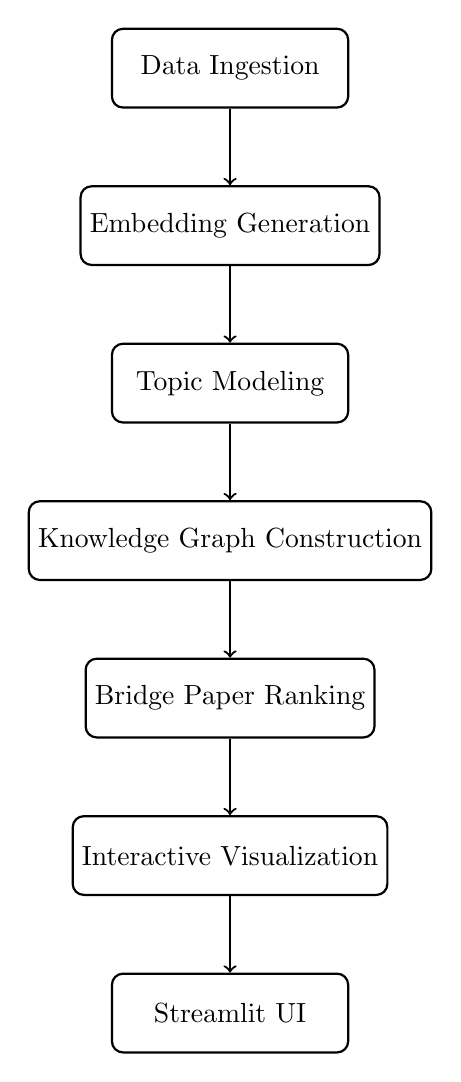
\begin{tikzpicture}[node distance=2cm, auto, thick]
    \node[draw, rectangle, rounded corners, minimum width=3cm, minimum height=1cm] (ingest) {Data Ingestion};
    \node[draw, rectangle, rounded corners, minimum width=3cm, minimum height=1cm, below of=ingest] (embed) {Embedding Generation};
    \node[draw, rectangle, rounded corners, minimum width=3cm, minimum height=1cm, below of=embed] (topic) {Topic Modeling};
    \node[draw, rectangle, rounded corners, minimum width=3cm, minimum height=1cm, below of=topic] (graph) {Knowledge Graph Construction};
    \node[draw, rectangle, rounded corners, minimum width=3cm, minimum height=1cm, below of=graph] (bridge) {Bridge Paper Ranking};
    \node[draw, rectangle, rounded corners, minimum width=3cm, minimum height=1cm, below of=bridge] (viz) {Interactive Visualization};
    \node[draw, rectangle, rounded corners, minimum width=3cm, minimum height=1cm, below of=viz] (ui) {Streamlit UI};
    
    \draw[->] (ingest) -- (embed);
    \draw[->] (embed) -- (topic);
    \draw[->] (topic) -- (graph);
    \draw[->] (graph) -- (bridge);
    \draw[->] (bridge) -- (viz);
    \draw[->] (viz) -- (ui);
\end{tikzpicture}
\caption{Paper Bridge Finder System Architecture}
\label{fig:architecture}
\end{figure}

\subsection{Component Overview}

\subsubsection{Data Ingestion}
The ingestion module fetches paper metadata from academic repositories like arXiv and Semantic Scholar based on specified research topics or paper IDs. It extracts titles, abstracts, authors, publication years, and citation information, creating a comprehensive dataset for analysis.

\subsubsection{Embedding Generation}
This component transforms paper abstracts into dense vector representations using SentenceTransformer, capturing the semantic meaning of each paper in a format suitable for machine learning algorithms.

\subsubsection{Topic Modeling}
The topic modeling module clusters papers into coherent research areas using K-means clustering on the embedded abstracts. Each cluster represents a distinct research topic, with automatically generated topic names based on frequent terms.

\subsubsection{Knowledge Graph Construction}
This component builds a graph representation of the paper ecosystem, with papers and topics as nodes, and various relationship types as edges (paper-topic membership, citations, cross-topic connections).

\subsubsection{Bridge Paper Ranking}
The ranking module identifies papers that effectively connect different topics, using metrics like shortest path distance, centrality measures, and paper recency to score potential bridge papers.

\subsubsection{Interactive Visualization}
The visualization component creates both static and interactive visualizations of the knowledge graph, clearly highlighting bridge papers with distinctive styling (orange-red borders and bridge emoji). All nodes are clickable in the interactive visualization, allowing direct access to the corresponding papers.

\subsubsection{Streamlit User Interface}
A user-friendly web interface built with Streamlit provides intuitive access to the system. Users can specify research areas, adjust parameters, and view results through multiple tabs displaying bridge papers, visualizations, and topic information.

\section{Methodology}

\subsection{Data Collection}

\subsubsection{Data Sources}
The system collects paper metadata from two primary sources:
\begin{itemize}
    \item \textbf{arXiv API}: Provides access to paper metadata including titles, abstracts, authors, and publication dates
    \item \textbf{Semantic Scholar API}: Supplements with citation information and additional metadata
\end{itemize}

\subsubsection{Metadata Extraction}
For each paper, the system extracts:
\begin{itemize}
    \item Paper ID (arXiv ID)
    \item Title
    \item Abstract
    \item Authors
    \item Publication year
    \item Citations (when available)
    \item URL
\end{itemize}

\subsubsection{Citation Network Building}
The system follows citation links to build a network of related papers, using a configurable "hop limit" to control the depth of exploration. When citation data is unavailable, the system simulates connections based on topic similarity.

\subsection{Text Representation}

\subsubsection{Embedding Technique}
The system uses the SentenceTransformer model (specifically \texttt{all-MiniLM-L6-v2}) to generate vector embeddings of paper abstracts. This model produces 384-dimensional vectors that capture the semantic meaning of each abstract.

\subsubsection{Quality Considerations}
The embedding quality directly impacts downstream tasks like topic modeling and similarity calculations. The chosen model balances quality with computational efficiency, providing good semantic representation while remaining lightweight enough for rapid processing.

\subsection{Topic Modeling}

\subsubsection{Clustering Approach}
The system uses K-means clustering on the normalized embeddings to group papers into coherent topics. This approach was chosen for its simplicity, efficiency, and interpretability compared to more complex methods like BERTopic.

\subsubsection{Topic Naming}
Topic names are automatically generated based on the most frequent meaningful terms in the titles of papers within each cluster. Stop words are filtered out to focus on domain-specific terminology.

\subsection{Knowledge Graph Construction}

\subsubsection{Node Types}
The knowledge graph contains two types of nodes:
\begin{itemize}
    \item \textbf{Paper nodes}: Representing individual academic papers
    \item \textbf{Topic nodes}: Representing clusters of related papers
\end{itemize}

\subsubsection{Edge Types}
Several types of edges connect the nodes:
\begin{itemize}
    \item \textbf{Paper-Topic edges} (type: \texttt{belongs\_to}, weight: 1.0): Connect papers to their assigned topics
    \item \textbf{Citation edges} (type: \texttt{cites}, weight: 0.7): Connect papers based on citation information
    \item \textbf{Same-Topic Similarity edges} (type: \texttt{similar\_topic}, weight: 0.5): Connect papers within the same topic when citation data is unavailable
    \item \textbf{Cross-Topic edges} (type: \texttt{cross\_topic}, weight: 0.3): Connect papers from different topics to enable bridge discovery
\end{itemize}

\subsection{Bridge Paper Identification}

\subsubsection{Ranking Algorithm}
The bridge ranking algorithm identifies papers that effectively connect different research topics by calculating a composite score based on several factors:

\begin{algorithm}[H]
\SetAlgoLined
\caption{Bridge Paper Ranking}
\KwData{paper, topic\_a, topic\_b}
\KwResult{bridge\_score}
$path\_a \gets$ ShortestPath(paper, topic\_a)\;
$path\_b \gets$ ShortestPath(paper, topic\_b)\;
$path\_length \gets |path\_a| + |path\_b|$\;
$centrality \gets$ BetweennessCentrality(paper)\;
$recency \gets$ RecencyScore(paper.year)\;
$connection\_strength \gets$ ConnectionStrength(paper)\;
$score \gets \alpha \cdot (1/path\_length) + \beta \cdot centrality + \gamma \cdot recency + \delta \cdot connection\_strength$\;
\Return{$score$}\;
\end{algorithm}

\subsubsection{Scoring Metrics}
The bridge score combines several metrics:
\begin{itemize}
    \item \textbf{Path distance}: How efficiently the paper connects the two topics
    \item \textbf{Centrality}: The paper's importance in the overall graph
    \item \textbf{Recency}: More recent papers are given higher weight
    \item \textbf{Connection strength}: The number and weight of connections the paper has
\end{itemize}

\section{Experimental Results}

\subsection{Example Research Combinations}
We tested the system with various research area combinations, including:
\begin{itemize}
    \item Quantum Computing and Machine Learning
    \item Materials Science and Quantum Computing
    \item Neuroscience and Reinforcement Learning
    \item Mechanical Engineering and Machine Learning
    \item Protein Folding and Machine Learning
\end{itemize}

In each case, the system successfully identified bridge papers that meaningfully connect the research domains.

\subsection{Dataset Statistics}
In our experiments with "quantum computing" and "machine learning", we processed a dataset with the following characteristics:
\begin{itemize}
    \item 30 papers (15 from each research area)
    \item 2 topic clusters
    \item 32 nodes in the knowledge graph (30 papers + 2 topics)
    \item Approximately 100 edges (30 paper-topic edges + citation/similarity edges)
\end{itemize}

\subsection{Topic Distribution Analysis}
The topic modeling produced the following clusters for one of our experiments:
\begin{table}[h]
\centering
\begin{tabular}{ccc}
\toprule
\textbf{Topic ID} & \textbf{Topic Name} & \textbf{Paper Count} \\
\midrule
0 & quantum + computing + computers & 15 \\
1 & learning + machine + deep & 15 \\
\bottomrule
\end{tabular}
\caption{Topic Distribution}
\label{tab:topics}
\end{table}

\subsection{Visualization Enhancements}
The knowledge graph visualization includes several key features:
\begin{itemize}
    \item \textbf{Bridge paper highlighting}: Papers connecting different domains are highlighted with orange-red borders and a bridge icon
    \item \textbf{Interactive exploration}: All nodes are clickable to open the corresponding papers directly
    \item \textbf{Color coding}: Different node types (papers, topics) and research areas use distinct colors
    \item \textbf{Both static and interactive formats}: Static PNG for quick viewing and interactive HTML for detailed exploration
\end{itemize}

\begin{figure}[htbp]
\centering
\fbox{
\begin{minipage}{0.8\textwidth}
\centering
\textbf{[Knowledge Graph Visualization]}\\
\vspace{0.5cm}
\textit{Visualization showing paper clusters and bridge papers connecting different research domains, with bridge papers highlighted with orange-red borders and bridge icon}
\end{minipage}
}
\caption{Enhanced Knowledge Graph Visualization}
\label{fig:graph_vis}
\end{figure}

\subsection{User Interface}
The system provides a user-friendly Streamlit interface that allows researchers to:
\begin{itemize}
    \item Enter two research areas to find connections between them
    \item View bridge papers ranked by their effectiveness in connecting domains
    \item Explore visualizations of the paper relationships
    \item Adjust parameters to refine search results
\end{itemize}

\section{Conclusion}

The Paper Bridge Finder addresses the important challenge of discovering connections between different research areas. By leveraging techniques from natural language processing, graph theory, and machine learning, the system automates the identification of papers that serve as bridges between topics.

Our experiments with various research area combinations demonstrate that the system can successfully identify meaningful connections between research domains, potentially accelerating interdisciplinary research and collaboration. The modular pipeline architecture ensures flexibility and extensibility, while the user-friendly Streamlit interface makes the system accessible to researchers without specialized technical knowledge.

The Paper Bridge Finder represents a step toward more connected and interdisciplinary research, helping researchers navigate the increasingly complex landscape of scientific literature and discover valuable connections across domain boundaries.

% --- End of main content ---

\end{document} 